\documentclass[../../D1.tex]{subfiles}

\begin{document}
\subsubsection{Neural Networks \& Deep Learning}

\begin{figure}[H]
    \centering
    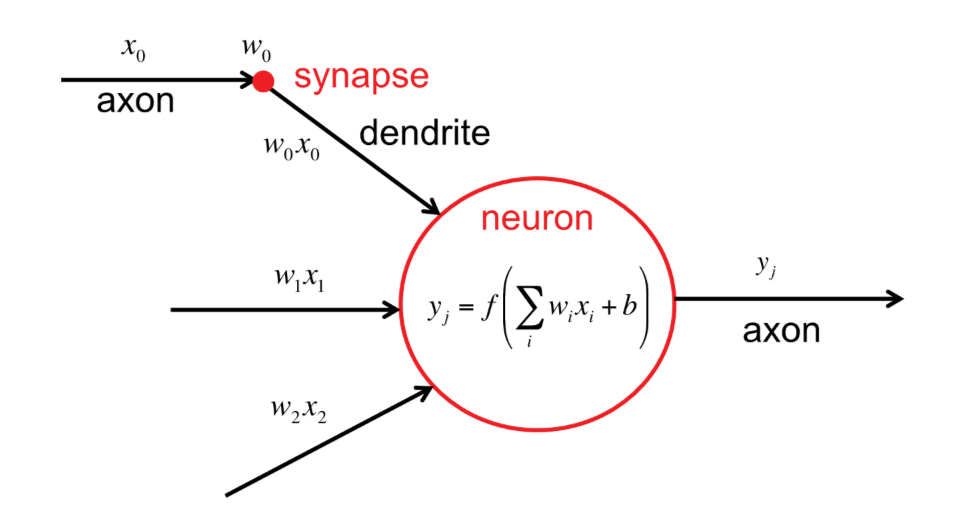
\includegraphics[width=0.6\textwidth]{Perceptron_efficient_proc.png}
    \caption{Neuron with corresponding biologically inspired labels.\\ \textbf{(Adopted figure from~\autocite{szeEfficientProcessingDeep2017})}}
    \label{fig:neuronLabeled}
\end{figure}
Deep learning is a subcategory of machine learning techniques where a hierarchy of layers perform some manner of information processsing with the goal of computing high level abstractions of the data by utilising low level abstractions identified in the early layers~\autocite{dengTutorialSurveyArchitectures2014}.


Neural networks fundamental purpose is to transform an input vector commonly referred to as~$X$ into an output vector~$\hat{Y}$. 
The output vector~$\hat{Y}$ is some form of classification such as a binary classification or a probability distribution over multiple classes~\autocite{thierry-miegHowFundamentalConcepts}. 
Between the input layer ($X$) and the output layer ($\hat{Y}$) there exists some number of interior layers that are referred to as hidden layers, the hidden and output layers are composed of neurons that pass signals derived from weights through the network, this model of computing was inspired by connectionism and our understanding of the human brain, see Fig.~\ref{fig:neuronLabeled} for labels of the analagous biological components. 
Weights in a neural network effectively correspond to the synapses in the brain and the output of the neruon is modelled as the axon. 
All neruons in a Neural network have weights corresponding to their inputs, these weights are are intended to mirror the value scaling effect of a synapse by performing a weighted sum operation~\autocite{szeEfficientProcessingDeep2017}.


Neural networks and deep neural networks are often reffered to interchangably, they are primarily distinguished by the number of layers, there is no hard rule indicating when a neural network is considered deep but generally a network with more than 3 hidden layers is considered a deep neural network, the rest of this dissertaion will refer to \acrshort{dnn}s for consistency. 
Each neuron in a \Acrshort{dnn} applies an non-linear activation function to the result of its weighted sum of inputs and randomly initialised weights, without which a \Acrshort{dnn} would just be a linear algebra operation~\autocite{szeEfficientProcessingDeep2017}, the cumulative effect of the activations in each layer results in elabourate causal chains of transormations that influence the aggregate activation of the network.

\subsubsection{Inference and Training}

\emph{Training} or learning in the context of DNNs is the process of finding the optimal parameters (value for the weights and bias) in the network.
Upon completion of training \emph{inference} can be performed, this is where new input data is fed into the network, a series of operations is performed using the trained parameters, and some meaninful output is obtained such as a classification, regression, or function approximation.
Many techniques can be used to search for optimal parameters, one example known as supervised learning is as follows: 
Begin by passing some training data through the network, next the gap between the known ideal output (labels) and the computed outputs from the current weights is calculated using a loss function. Finally the weights are updated using an optimization process such as gradient descent coupled with some form of backward pass, backpropagation is a popular choice for this.



\subsubsection{Convolutional Neural Networks}

Much like traditional nerual networks the \Acrshort{cnn} architecture was inspired by human and animal brains, the concept of processing the input with local receptive fields is conceptually similar some functionality of the cat's visual cortex~\autocite{hubelReceptiveFieldsBinocular1962,lecunConvolutionalNetworksImages,pouyanfarSurveyDeepLearning2019}. 
The influential paper by Hubel \& Weisel~\autocite{hubelReceptiveFieldsBinocular1962} ultimately had a significant influence on the design of \Acrshort{cnn}s via the Neocognitron, as proposed by Fukushima in~\autocite{fukushimaNeocognitronSelforganizingNeural1980} and again evaluated in~\autocite{fukushimaNeocognitronHierarchicalNeural1988}, these papers paved the way for the modern CNN. 

A critical aspect of image recognition is robustness to input shift and distortion, this robustness was indicated as one of the primary achivements of the Neocognitron in Fukushima's paper~\autocite{fukushimaNeocognitronSelforganizingNeural1980}. LeCunn and Bengio provide comprehensive explainations of how traditional \acrshort{dnn}s are so inefficient for these tasks 


The local receptive fields enable neurons to extract low level features such as edges, corners, and end-points with respect to their orientation. 
\Acrshort{cnn}s are robust to input shift or distortion by using receptive fields to identify these low level features across the entire input space, performing local averaging and downsampling in the layers following convolution layers means the absolute location of the features is less important than the position of the features relative to the position of other identified features~\autocite{lecunConvolutionalNetworksImages}. 
Each layer produces higher degrees of abstraction from the input layer, in doing so these abstractions retain important information about the input, these abstractions are referred to as feature maps.
The layers performing downsampling are known as pooling layers, they reduce the resolution or dimensions of the feature map which reduces overfitting and speeds up training by reducing the number of parameters in the network~\autocite{pouyanfarSurveyDeepLearning2019}.


\acrshort{cnn}s have been found to be effective in many different AI domains, popular applications include: computer vision, \Acrshort{nlp}, and speech processing. 
However they are notorious for needing careful tuning of various hyperparameters, it is often computationally intensive to exhaustively search for optimal CNN hyperparameters, Snoek et al.~\autocite{snoekPracticalBayesianOptimization2012} sucessfully applied a bayesian optimisation algorithm to efficiently search for higher quality hyperparameters.

\begin{figure}
    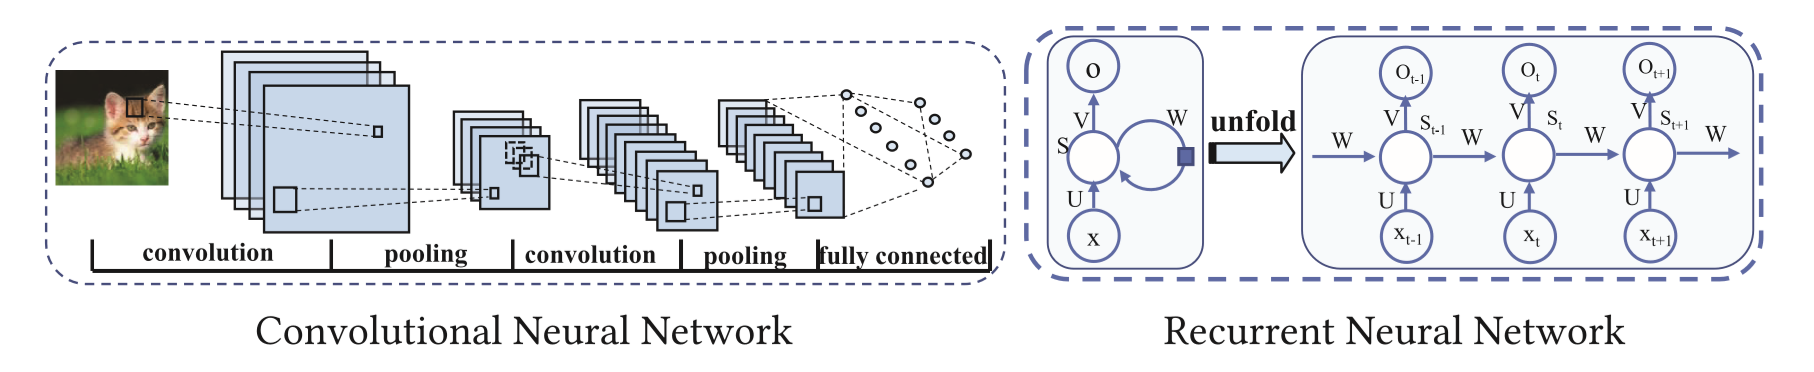
\includegraphics[width=1\textwidth]{CNN_RNN.png} 
    \caption{A typical example of a \acrshort*{cnn} (left) and \acrshort{rnn} (right)\\ \textbf{(Adopted figure from~\autocite{chenDeepLearningMobile2020})}}
    \label{fig:exampleCnnRnn}   
\end{figure}

\newpage
\subsubsection{Filters and Feature Maps}

\newpage

\end{document}